\documentclass[10pt,a4paper]{article}
\usepackage[utf8]{inputenc}
\usepackage{amsmath}
\usepackage{amsfonts}
\usepackage{amssymb}
\usepackage{float}
\usepackage{graphicx}
\usepackage[left=2cm,right=2cm,top=2cm,bottom=2cm]{geometry}
\usepackage{parskip}
\author{Songtuan Lin u6162630}
\title{Assignment 2}
\begin{document}
\maketitle
\section*{Question 1}
According to the definition of norm, the equation $\| \mathbf{x} - \mathbf{x_{0}} \|_{2} \leq \| \mathbf{x} - \mathbf{x_{1}} \|_{2}$ is the same as:
\begin{equation*}
	(\mathbf{x} - \mathbf{x_{0}})^{T} (\mathbf{x} - \mathbf{x_{0}}) \leq (\mathbf{x} - \mathbf{x_{1}})^{T} (\mathbf{x} - \mathbf{x_{1}})
\end{equation*}
Which can be further expressed as:
\begin{equation}
	\mathbf{x}^{T} (\mathbf{x_{1}} - \mathbf{x_{0}}) + (\mathbf{x_{1}} - \mathbf{x_{0}})^{T} \mathbf{x} \leq \mathbf{x_{1}}^{T} \mathbf{x_{1}} - \mathbf{x_{0}}^{T} \mathbf{x_{0}}
	\label{1}
\end{equation}
Since $\mathbf{x}^{T} (\mathbf{x_{1}} - \mathbf{x_{0}}) = \big( (\mathbf{x_{1}} - \mathbf{x_{0}})^{T} \mathbf{x} \big)^{T}$, which produce a constant, we have:
\begin{equation}
	\mathbf{x}^{T} (\mathbf{x_{1}} - \mathbf{x_{0}}) = (\mathbf{x_{1}} - \mathbf{x_{0}})^{T} \mathbf{x}
	\label{2}
\end{equation} 
Replace equation \ref{2} to equation \ref{1}, there is:
\begin{equation*}
	2 (\mathbf{x_{1}} - \mathbf{x_{0}})^{T} \mathbf{x} \leq \mathbf{x_{1}}^{T} \mathbf{x_{1}} - \mathbf{x_{0}}^{T} \mathbf{x_{0}}
\end{equation*}
Which follow the definition of half-space: $\mathbf{\lambda}^{T} \mathbf{x} \leq \mathbf{b}$, where $\mathbf{\lambda} = 2 (\mathbf{x_{1}} - \mathbf{x_{0}})$ and $\mathbf{b} = \mathbf{x_{1}}^{T} \mathbf{x_{1}} - \mathbf{x_{0}}^{T} \mathbf{x_{0}}$.

\section*{Question 2}
The polyhedron constructed by the convex hull is the area with the 5 color line as boundary, shown in following figure:
\begin{figure}[H]
	\begin{center}
		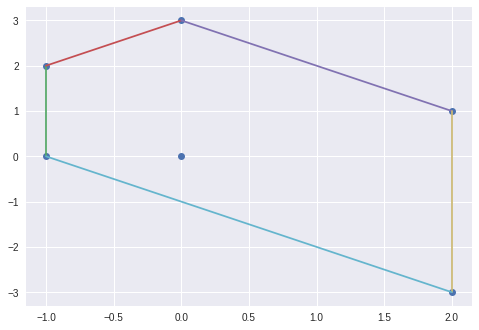
\includegraphics[scale=0.4]{Q2.png}
	\end{center}
\end{figure}
Denote $\mathbf{x} = \begin{bmatrix}
x_{1} \\
x_{2}
\end{bmatrix}$ as the point within $\mathcal{R}^{2}$, the hyper-plane defined by the 5 color line shown in above figure are:
\begin{equation*}
	\begin{bmatrix}
		-1 & 0 \\
		1 & 1 \\
		1 & 0 \\
		1 & 1
	\end{bmatrix} \mathbf{x} = 
	\begin{bmatrix}
		-1 \\
		-1 \\
		2 \\
		3
	\end{bmatrix}
\end{equation*}
As a result, the polyhedron constructed by these hyper-plane can be expressed as:
\begin{equation*}
	\mathcal{A} \mathbf{x} \preceq \mathbf{b}
\end{equation*}
Where $\mathcal{A} = \begin{bmatrix}
1 & 0 \\
1 & 1 \\
1 & 0 \\
1 & 1
\end{bmatrix}$ and $\mathbf{b} = \begin{bmatrix}
-1 \\
-1 \\
2 \\
3
\end{bmatrix}$

\section*{Question 3}

\subsection*{(a)}
Denote set $\{ \mathbf{x} |\, \alpha \leq \mathbf{a}^{T}\mathbf{x} \leq \beta \}$ as $\mathcal{C}$, then, $\mathcal{C}$ is a convex set. The prove is as follow:

Assume $\mathbf{x_{1}}, \mathbf{x_{2}} \in \mathcal{C}$, their convex combination follow:
\begin{equation}
	\mathbf{a}^{T}(\theta \mathbf{x_{1}} + (1 - \theta) \mathbf{x_{2}}) = \theta \mathbf{a}^{T} \mathbf{x} + (1 - \theta) \mathbf{a}^{T} \mathbf{x_{2}}
	\label{3}
\end{equation}
Since $\mathbf{x_{1}}, \mathbf{x_{2}} \in \mathcal{C}$, there is:
\begin{equation}
	\begin{cases}
		\mathbf{a}^{T} \mathbf{x_{1}} \geq \alpha \\
		\mathbf{a}^{T} \mathbf{x_{2}} \geq \alpha
	\end{cases}
	\label{4}
\end{equation}
Combine equation \ref{3} and \ref{4}, we have:
\begin{align*}
	\theta \mathbf{a}^{T} \mathbf{x} + (1 - \theta) \mathbf{a}^{T} \mathbf{x_{2}} &\geq \theta \alpha + (1 - \theta) \alpha \\
	&= \alpha
\end{align*}
The equation $\theta \mathbf{a}^{T} \mathbf{x} + (1 - \theta) \mathbf{a}^{T} \mathbf{x_{2}} \leq \beta$ can be proved by using the same method. As a result, when $\mathbf{x_{1}}, \mathbf{x_{2}} \in \mathcal{C}$, $\theta \mathbf{x_{1}} + (1 - \theta) \mathbf{x_{2}} \in \mathcal{C}$ hold for any $0 \leq \theta \leq 1$. Thus, $\mathcal{C}$ is a convex set.

\subsection*{(b)}
The \textit{rectangle} set $\mathcal{G}$ can be thought as the intersection of different sets that follow:
\begin{equation*}
	\mathcal{G} = \displaystyle\bigcap_{i = 1}^{n} \mathcal{G}_{i}
\end{equation*}
Where $\mathcal{G}_{i}$ is the set: $\{ \mathbf{x} |\, \alpha \leq x_{i} \leq \beta \}$. It is obvious that $\mathcal{G}_{i}$ is the \textit{slab} defined in (a) with 
\begin{equation*}
	\mathbf{a} = 
	\begin{bmatrix}
		0 \\
		\vdots \\
		1 \\
		\vdots \\
		0
	\end{bmatrix}
\end{equation*}
In which, the ith element $a_{i}$ that corresponding to $x_{i}$ within $\mathbf{x}$ is set to be 1 and the other elements is 0. Therefore, $\mathcal{G}_{i}$ is convex, which means, $\mathcal{G}$ is the intersection of convex set, which is also convex. 

\subsection*{(c)}
The set $\{ \mathbf{x} |\, \mathbf{a_{1}}^{T} \mathbf{x} \leq b_{1}, \mathbf{a_{2}}^{T} \mathbf{x} \leq b_{2} \}$ is the same as:
\begin{equation*}
\{ \mathbf{x} |\, \mathbf{a_{1}}^{T} \mathbf{x} \leq b_{1} \} \cap \{ \mathbf{x} |\, \mathbf{a_{2}}^{T} \mathbf{x} \leq b_{2} \}
\end{equation*}
For any $i \in \{ 0, 1 \}$, the set $\{ \mathbf{x} |\, \mathbf{a_{i}}^{T} \mathbf{x} \leq b_{i} \}$ define a half-space, which is a convex set. As a result, the set $\{ \mathbf{x} |\, \mathbf{a_{1}}^{T} \mathbf{x} \leq b_{1}, \mathbf{a_{2}}^{T} \mathbf{x} \leq b_{2} \}$ is the intersection of two convex set, which is also convex.

\subsection*{(d)}
Assume $\mathcal{S} = \{ \mathbf{s_{1}}, \mathbf{s_{2}}, \cdots, \mathbf{s_{n}} \}$. The original set $\{ \mathbf{x} |\, \| \mathbf{x} - \mathbf{x_{0}} \|_{2} \leq \| \mathbf{x} - \mathbf{s} \|_{2} \text{ for any } \mathbf{s} \in \mathcal{S} \}$ can be expressed as:
\begin{equation*}
	\displaystyle\bigcap_{i = 1}^{n}\{ \mathbf{x} |\, \| \mathbf{x} - \mathbf{x_{0}} \|_{2} \leq \| \mathbf{x} - \mathbf{s_{i}} \|_{2} \}
\end{equation*}
The same concept can be expanded to set $\mathcal{S}$ which has infinite element($n \rightarrow \infty$). According to Question 1, the single set $\mathbf{x} |\, \| \mathbf{x} - \mathbf{x_{0}} \|_{2} \leq \| \mathbf{x} - \mathbf{s_{i}} \|_{2}$ define a half-space and is convex. As a result, the intersection of these convex is also convex, which means, $\{ \mathbf{x} |\, \| \mathbf{x} - \mathbf{x_{0}} \|_{2} \leq \| \mathbf{x} - \mathbf{s} \|_{2} \text{ for any } \mathbf{s} \in \mathcal{S} \}$ is convex.

\subsection*{(e)}
We first consider the set:
\begin{equation}
	\mathcal{G}_{i} = \{ \mathbf{x} |\, \| \mathbf{x} - \mathbf{s_{i}} \|_{2} \leq \| \mathbf{x} - \mathbf{s} \|_{2} \textit{ for all } \mathbf{s} \in \mathcal{S} \}
	\label{5}
\end{equation}
Where $\mathbf{s_{i}} \in \mathcal{S}$ is a fixed point within $\mathcal{S}$. This set is consist of points $\mathbf{x}$ that have the minimum distance to $\mathcal{S}$ through $\mathbf{s_{i}}$. It is obvious that
\begin{equation}
	\{ \mathbf{x} |\, \| \mathbf{x} - \mathbf{s_{i}} \|_{2} \leq \| \mathbf{x} - \mathbf{s} \|_{2} \} \cap \{ \mathbf{x} |\, \| \mathbf{x} - \mathbf{s_{j}} \|_{2} \leq \| \mathbf{x} - \mathbf{s} \|_{2} \} = \emptyset
	\label{6}
\end{equation}
when $\mathbf{s_{i}}, \mathbf{s_{j}} \in \mathcal{S}$ and $\mathbf{s_{i}} \neq \mathbf{s_{j}}$ as a point $\mathbf{x}$ can only achieve the minimum distance to $\mathcal{S}$ by hold $\| \mathbf{x} - \mathbf{s_{i}} \| < \| \mathbf{x} - \mathbf{s_{j}} \|$ or the inverse. Now assume $\mathcal{S} = \{ \mathbf{s_{1}}, \mathbf{s_{2}}, \cdots, \mathbf{s_{n}} \}$ and $\mathcal{T} = \{ \mathbf{t_{1}}, \mathbf{t_{2}}, \cdots, \mathbf{t_{k}} \}$. We define the set:
\begin{equation*}
	\mathcal{Q}_{i} = \{ \mathbf{x} |\, \| \mathbf{x} - \mathbf{s_{i}} \|_{2} \leq \| \mathbf{x} - \mathbf{t} \|_{2} \textit{ for all } \mathbf{t} \in \mathcal{T} \}
\end{equation*}
Where $\mathbf{s_{i}} \in \mathcal{S}$. This set describe the point $\mathbf{x}$ that the distance between $\mathbf{x}$ and a point $\mathbf{s_{i}} \in \mathcal{S}$ is less than the distance between $\mathbf{x}$ and set $\mathcal{T}$. As a result, the set $\{ \mathbf{x} |\, \textbf{dist}(\mathbf{x}, \mathcal{S}) < \textbf{dist}(\mathbf{x}, \mathcal{T}) \}$ can be then expressed as:
\begin{equation*}
	\displaystyle\bigcup_{i = 1}^{n}(\mathcal{G}_{i} \cap \mathcal{Q}_{i})
\end{equation*}
According to equation \ref{6}, for any $1 \leq i, j \leq n$, $\mathcal{G}_{i} \cap \mathcal{G}_{j} = \emptyset$. Hence, $(\mathcal{G}_{i} \cap \mathcal{Q}_{i}) \cup (\mathcal{G}_{j} \cap \mathcal{Q}_{j}) = \emptyset$, which means, the set $\{ \mathbf{x} |\, \textbf{dist}(\mathbf{x}, \mathcal{S}) < \textbf{dist}(\mathbf{x}, \mathcal{T}) \}$  is separated and therefore can not be convex.

\subsection*{(f)}
Assume $\mathcal{S}_{1} = \{ \mathbf{s_{1}}, \mathbf{s_{2}}, \cdots, \mathbf{s_{n}} \}$. Then, the set $\mathcal{C} =  \{ \mathbf{x} |\, \mathbf{x} + \mathcal{S}_{1} \subset \mathcal{S}_{2} \}$ can be replaced as the intersection of different set as:
\begin{equation*}
	\mathcal{C} = \displaystyle\bigcap_{i = 1}^{n}\mathcal{C}_{i}
\end{equation*}
Where $\mathcal{C}_{i} = \{ \mathbf{x} |\, \mathbf{x} + \mathbf{s_{i}} \in \mathcal{S}_{2} \}$. It can be proved that $\mathcal{C}_{i}$ is convex: Assume $\mathbf{x_{1}}, \mathbf{x_{2}} \in \mathcal{C}_{i}$. The equation $\theta \mathbf{x_{1}} + (1 - \theta) \mathbf{x_{2}} + \mathbf{s_{i}}$ can be expressed as:
\begin{equation*}
	\theta \mathbf{x_{1}} + (1 - \theta) \mathbf{x_{2}} + \mathbf{s_{i}} = \theta(\mathbf{x_{1}} + \mathbf{s_{i}})  + (1 - \theta) (\mathbf{x}_{2} + \mathbf{s_{i}})
\end{equation*}
Since $\mathbf{x_{1}} + \mathbf{s_{i}}, \mathbf{x_{2}} + \mathbf{s_{i}} \in \mathcal{S}_{2}$ and $\mathcal{S}_{2}$ is convex, we have $\theta(\mathbf{x_{1}} + \mathbf{s_{i}})  + (1 - \theta) (\mathbf{x}_{2} + \mathbf{s_{i}}) \in \mathcal{S}_{2}$. Hence, $\mathcal{C}_{i}$ is convex. As a result, $\mathcal{C}$ is convex as it is the intersection of convex set.

\subsection*{(g)}
The equation $\| \mathbf{x} - \mathbf{a} \|_{2} \leq \theta \| \mathbf{x} - \mathbf{b} \|_{2}$ is the same as $\| \mathbf{x} - \mathbf{a} \|^{2}_{2} \leq \theta^{2} \| \mathbf{x} - \mathbf{b} \|^{2}_{2}$. Now, let $\theta^{2} = p$, the equation mentioned before can be expanded as:
\begin{equation}
	\mathbf{x}^{T}\mathbf{x} + \frac{2 (p \mathbf{b} - \mathbf{a})^{T}}{1 - p} \mathbf{x} + \frac{\mathbf{a}^{T} \mathbf{a} - p \mathbf{b}^{T}\mathbf{b}}{1 - p} \leq 0
	\label{7}
\end{equation}
Which has the same form as the equation that describe a ball:
\begin{equation}
	\| \mathbf{x} - \mathbf{x_{0}} \|^{2}_{2} = \mathbf{x}^{T} \mathbf{x} - 2 \mathbf{x_{0}}^{T} \mathbf{x} + \mathbf{x_{0}}^{T} \mathbf{x_{0}} \leq r^{2}
	\label{8}
\end{equation}
Compare equation \ref{7} with \ref{8}, it is easy to figure out that:
\begin{equation*}
	\mathbf{x_{0}} = \frac{\mathbf{a} - p \mathbf{b}}{1 - p} \textit{ and } r^{2} = \mathbf{x_{0}}^{T} \mathbf{x_{0}} - \frac{\mathbf{a}^{T} \mathbf{a} - p \mathbf{b}^{T} \mathbf{b}}{1 - p}
\end{equation*}
If $r^{2} \geq 0 $ can be verified, then, equation \ref{7} always describe a ball. Indeed, $r^{2}$ can be expanded as:
\begin{equation*}
	r^{2} = \frac{(\mathbf{a} - p \mathbf{b})^{T} (\mathbf{a} - p \mathbf{b})}{(1 - p)^{2}} - \frac{\mathbf{a}^{T} \mathbf{a} - p \mathbf{b}^{T} \mathbf{b}}{1 - p}
\end{equation*}
Which is the same as:
\begin{equation*}
	r^{2} = \frac{p(\mathbf{a}^{T} \mathbf{a} - 2 \mathbf{a}^{T} \mathbf{b} + \mathbf{b}^{T} \mathbf{b})}{(1 - p)^{2}}
\end{equation*}
Since $\mathbf{a}^{T} \mathbf{a} - 2 \mathbf{a}^{T}\mathbf{b} + \mathbf{b}^{T} \mathbf{b} = \| \mathbf{a} - \mathbf{b} \|^{2}_{2} \geq 0$, $r^{2}$ is also greater or equal to zero. Hence, equation \ref{7} describe a ball, which is a convex set.
\end{document}